%% 
%% Latex template to System Architecture Document
%% Author: Dario A. Palminio
%% LaTeX version 2.0
%% OS: Ubuntu
%% Editor: LaTeXila 2.4.0
%% 

\documentclass[a4paper,11pt]{book}
\usepackage[T1]{fontenc}
\usepackage[utf8]{inputenc}
\usepackage{lmodern}
\usepackage{graphicx}

\graphicspath{ {images/} }

\title{Daro Generic Persistence v1.0 - Software Architecture}
\author{Dario A. Palminio}

\begin{document}

\maketitle
Licence: Creative Commons by-sa 4.0
\newline
https://creativecommons.org/licenses/by-sa/4.0/
\newline

Documentation control

%% Document Version Control (Table)
\begin{table}[h]
\begin{tabular}{lllll}
\cline{1-4}
\multicolumn{1}{|l|}{Date}       & \multicolumn{1}{l|}{Author}         & \multicolumn{1}{l|}{Version} & \multicolumn{1}{l|}{Detail}   &  \\ \cline{1-4}
\multicolumn{1}{|l|}{05/05/2015} & \multicolumn{1}{l|}{Dario Palminio} & \multicolumn{1}{l|}{1.0}     & \multicolumn{1}{l|}{Creation} &  \\ \cline{1-4}
\multicolumn{1}{|l|}{04/06/2015} & \multicolumn{1}{l|}{Dario Palminio} & \multicolumn{1}{l|}{1.0}     & \multicolumn{1}{l|}{Add info} &  \\ \cline{1-4}
\multicolumn{1}{|l|}{06/06/2015} & \multicolumn{1}{l|}{Dario Palminio} & \multicolumn{1}{l|}{1.0}     & \multicolumn{1}{l|}{Add integration section} &  \\ \cline{1-4}
                                 &                                     &                              &                               &  \\
                                 &                                     &                              &                               & 
\end{tabular}
\end{table}
%% 

\tableofcontents

\chapter{Introduction}
Generic Persistence is un component (package) that implements CRUD (Create, read, update and delete) into DAO (Data Access Object) Generic Persistence in Java. This component uses Hibernate as an Object-Relational Mapping (ORM) framework, Hibernate is concerned with data persistence as it applies to relational databases (via JDBC). This component was designed to deliver a highly scalable architecture and reuse capability. This is configurable and extensible. This integrate hibernate with Spring application. With Hibernate framework, we provide all the database information using anotations and files. We can provide all the information (data source, JDBC connector and mapping) in an Application Context file (xml) from application that uses this library component.

The advantage of using this library component is the relatively simple and rigorous separation between two important parts of an application that can but should not know anything of each other, and which can be expected to evolve frequently and independently. This library component act as an intermediary between the application and the database persistence (CRUD generic on DAO).

\section{Purpose of the document}
The purpose of this document is to show the general architecture of a Java component called "Daro Generic Persistence".

\section{Audience}
Because the document is public license (Creative Commons by-sa 4.0) it was written for anyone interested audience.

\chapter{Architecture}
% text

\section{Scope and Context}
The Generic Persistence component consists of a JAR package ("com.daro.persistence.generic") named "DaroGenericPersistence-<VERSION>.jar" that can be used from other applications ("Concrete Persistence Service" or application) by extending the core classes.

\begin{figure}[h] % Diagram
  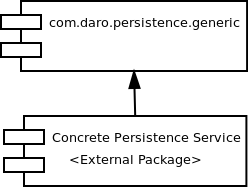
\includegraphics{generic_persistence_package_diagram}
  \caption{Context Diagram - Package Diagram}
  \centering
  \label{fig:context} %\ref{fig:context}
\end{figure}

\section{High-level Architecture}
% text

\pagebreak
\subsubsection{Class Diagram}
The classes described below belong to the package named "com.daro.persistence.generic".

\begin{figure}[h] % Diagram
  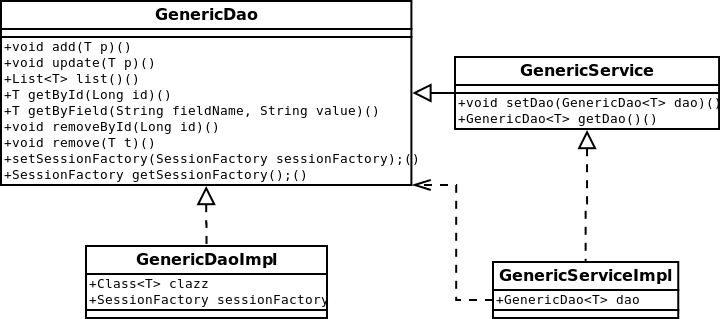
\includegraphics[width=\textwidth]{generic_persistence_class_diagram}
  \caption{General class diagram - high level}
  \centering
  \label{fig:generic_persistence_class_diagram} %\ref{fig:generic_persistence_class_diagram}
\end{figure}

\pagebreak
\subsubsection{Example of a Simple Client}
Here's a way to use the component. This example corresponds to the component testing.
To use of simple manner the library from code is necessary to extend the GenericDaoImpl class with an entity class (POJO).
For example, to persist an entity named PersonEntity can use a class named PersonPersistence that extends GenericDaoImpl.
The example shown in the following diagram:

\begin{figure}[h] % Diagram
  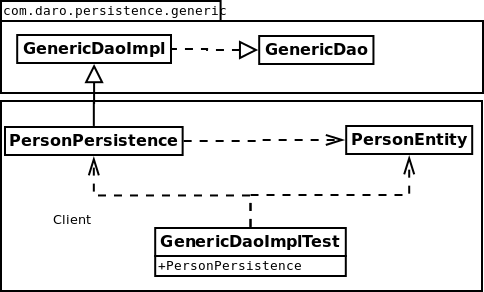
\includegraphics[width=\textwidth]{generic_persistence_class_diagram_to_use_simple}
  \caption{Example of how to use on simple manner - diagram}
  \centering
  \label{fig:generic_persistence_class_diagram_to_use_simple} %\ref{fig:generic_persistence_class_diagram_to_use_simple}
\end{figure}

\pagebreak
\subsubsection{Example of a Complex Client}
Here's a way to use the component. This example corresponds to the component testing.
The component can also be used in a more complex manner which allows greater scalability. 
This way is using the services layer. This requires extending the DAO class and Service class.
The example is shown in the following diagram:

\begin{figure}[h] % Diagram
  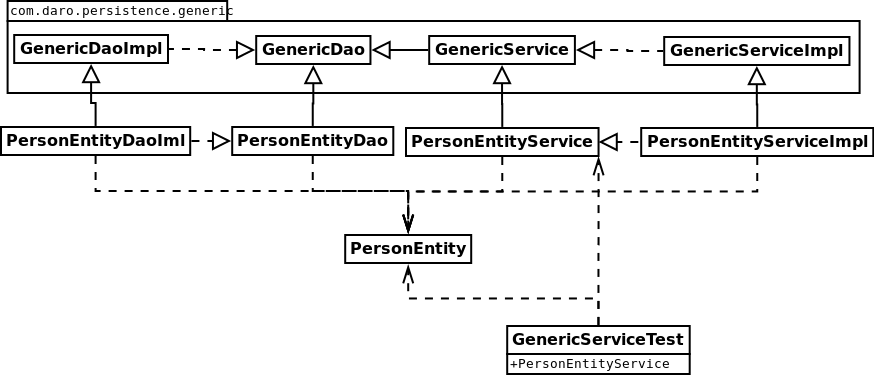
\includegraphics[width=\textwidth]{generic_persistence_class_diagram_to_use}
  \caption{Example of how to use - diagram}
  \centering
  \label{fig:generic_persistence_class_diagram_to_use} %\ref{fig:generic_persistence_class_diagram_to_use}
\end{figure}

\pagebreak
\subsection{Integration}
The integration is importing this library and configure it via spring application context file (For example you can see test-spring-context.xml file).

The steps required to integrate the library into a java project are:

\begin{itemize}
\item Import library into java project.
\item Add database connector driver (for example mysql-connector-java).
\item To inject DataSourse (via spring application context file).
\item To inject SessionFactory and set each entity to be recognized by the SessionFactory (via spring application context file).
\item To inject Transaction Manager (via spring application context file).
\item Inject SessionFactory each Class Dao we use in the project.
\end{itemize}

The classes are integrated with Hibernate-Spring as shown in the diagram:

\begin{figure}[h] % Diagram
  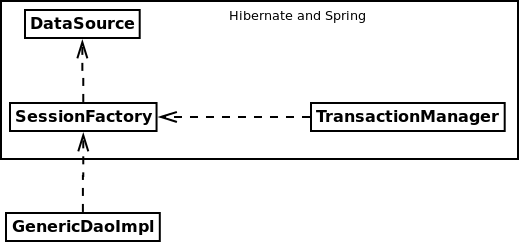
\includegraphics[width=\textwidth]{generic_persistence_integration_diagram}
  \caption{Hibernate-Spring Integration diagram}
  \centering
  \label{fig:generic_persistence_integration_diagram} %\ref{fig:generic_persistence_integration_diagram}
\end{figure}

\end{document}
